% Options for packages loaded elsewhere
\PassOptionsToPackage{unicode}{hyperref}
\PassOptionsToPackage{hyphens}{url}
%
\documentclass[
]{article}
\usepackage{lmodern}
\usepackage{amssymb,amsmath}
\usepackage{ifxetex,ifluatex}
\ifnum 0\ifxetex 1\fi\ifluatex 1\fi=0 % if pdftex
  \usepackage[T1]{fontenc}
  \usepackage[utf8]{inputenc}
  \usepackage{textcomp} % provide euro and other symbols
\else % if luatex or xetex
  \usepackage{unicode-math}
  \defaultfontfeatures{Scale=MatchLowercase}
  \defaultfontfeatures[\rmfamily]{Ligatures=TeX,Scale=1}
\fi
% Use upquote if available, for straight quotes in verbatim environments
\IfFileExists{upquote.sty}{\usepackage{upquote}}{}
\IfFileExists{microtype.sty}{% use microtype if available
  \usepackage[]{microtype}
  \UseMicrotypeSet[protrusion]{basicmath} % disable protrusion for tt fonts
}{}
\makeatletter
\@ifundefined{KOMAClassName}{% if non-KOMA class
  \IfFileExists{parskip.sty}{%
    \usepackage{parskip}
  }{% else
    \setlength{\parindent}{0pt}
    \setlength{\parskip}{6pt plus 2pt minus 1pt}}
}{% if KOMA class
  \KOMAoptions{parskip=half}}
\makeatother
\usepackage{xcolor}
\IfFileExists{xurl.sty}{\usepackage{xurl}}{} % add URL line breaks if available
\IfFileExists{bookmark.sty}{\usepackage{bookmark}}{\usepackage{hyperref}}
\hypersetup{
  pdftitle={Economic and government transfer variables, actual and projected, 2007-2030},
  hidelinks,
  pdfcreator={LaTeX via pandoc}}
\urlstyle{same} % disable monospaced font for URLs
\usepackage[margin=1in]{geometry}
\usepackage{graphicx}
\makeatletter
\def\maxwidth{\ifdim\Gin@nat@width>\linewidth\linewidth\else\Gin@nat@width\fi}
\def\maxheight{\ifdim\Gin@nat@height>\textheight\textheight\else\Gin@nat@height\fi}
\makeatother
% Scale images if necessary, so that they will not overflow the page
% margins by default, and it is still possible to overwrite the defaults
% using explicit options in \includegraphics[width, height, ...]{}
\setkeys{Gin}{width=\maxwidth,height=\maxheight,keepaspectratio}
% Set default figure placement to htbp
\makeatletter
\def\fps@figure{htbp}
\makeatother
\setlength{\emergencystretch}{3em} % prevent overfull lines
\providecommand{\tightlist}{%
  \setlength{\itemsep}{0pt}\setlength{\parskip}{0pt}}
\setcounter{secnumdepth}{-\maxdimen} % remove section numbering
\ifluatex
  \usepackage{selnolig}  % disable illegal ligatures
\fi

\title{Economic and government transfer variables, actual and projected,
2007-2030}
\author{}
\date{\vspace{-2.5em}}

\begin{document}
\maketitle

\begin{verbatim}
## Warning: package 'tidyverse' was built under R version 4.0.2
\end{verbatim}

\begin{verbatim}
## Warning: package 'ggplot2' was built under R version 4.0.2
\end{verbatim}

\begin{verbatim}
## Warning: package 'tibble' was built under R version 4.0.2
\end{verbatim}

\begin{verbatim}
## Warning: package 'tidyr' was built under R version 4.0.2
\end{verbatim}

\begin{verbatim}
## Warning: package 'readr' was built under R version 4.0.2
\end{verbatim}

\begin{verbatim}
## Warning: package 'purrr' was built under R version 4.0.2
\end{verbatim}

\begin{verbatim}
## Warning: package 'dplyr' was built under R version 4.0.2
\end{verbatim}

\begin{verbatim}
## Warning: package 'stringr' was built under R version 4.0.2
\end{verbatim}

\begin{verbatim}
## Warning: package 'forcats' was built under R version 4.0.2
\end{verbatim}

\begin{verbatim}
## Warning: package 'reshape2' was built under R version 4.0.2
\end{verbatim}

\begin{verbatim}
## Warning: package 'zoo' was built under R version 4.0.2
\end{verbatim}

\begin{verbatim}
## Warning: package 'quantmod' was built under R version 4.0.2
\end{verbatim}

\begin{verbatim}
## Warning: package 'xts' was built under R version 4.0.2
\end{verbatim}

\begin{verbatim}
## Warning: package 'TTR' was built under R version 4.0.2
\end{verbatim}

\begin{verbatim}
## Warning: package 'data.table' was built under R version 4.0.2
\end{verbatim}

\begin{verbatim}
## Warning: package 'lubridate' was built under R version 4.0.2
\end{verbatim}

\begin{verbatim}
## Warning: package 'Hmisc' was built under R version 4.0.2
\end{verbatim}

\begin{verbatim}
## Warning: package 'survival' was built under R version 4.0.2
\end{verbatim}

\begin{verbatim}
## Warning: package 'magrittr' was built under R version 4.0.2
\end{verbatim}

\begin{verbatim}
## Warning: package 'readxl' was built under R version 4.0.2
\end{verbatim}

\begin{verbatim}
## Warning: package 'writexl' was built under R version 4.0.2
\end{verbatim}

\begin{verbatim}
## Warning: package 'ggthemes' was built under R version 4.0.2
\end{verbatim}

\begin{verbatim}
## Warning: package 'ggtext' was built under R version 4.0.2
\end{verbatim}

\begin{verbatim}
## Warning: package 'gridExtra' was built under R version 4.0.2
\end{verbatim}

\begin{verbatim}
## Warning: package 'wesanderson' was built under R version 4.0.2
\end{verbatim}

\begin{verbatim}
## Warning: package 'tinytex' was built under R version 4.0.2
\end{verbatim}

\hypertarget{projected-nominal-government-consumption-and-investment}{%
\section{Projected Nominal Government Consumption and
Investment}\label{projected-nominal-government-consumption-and-investment}}

\begin{center}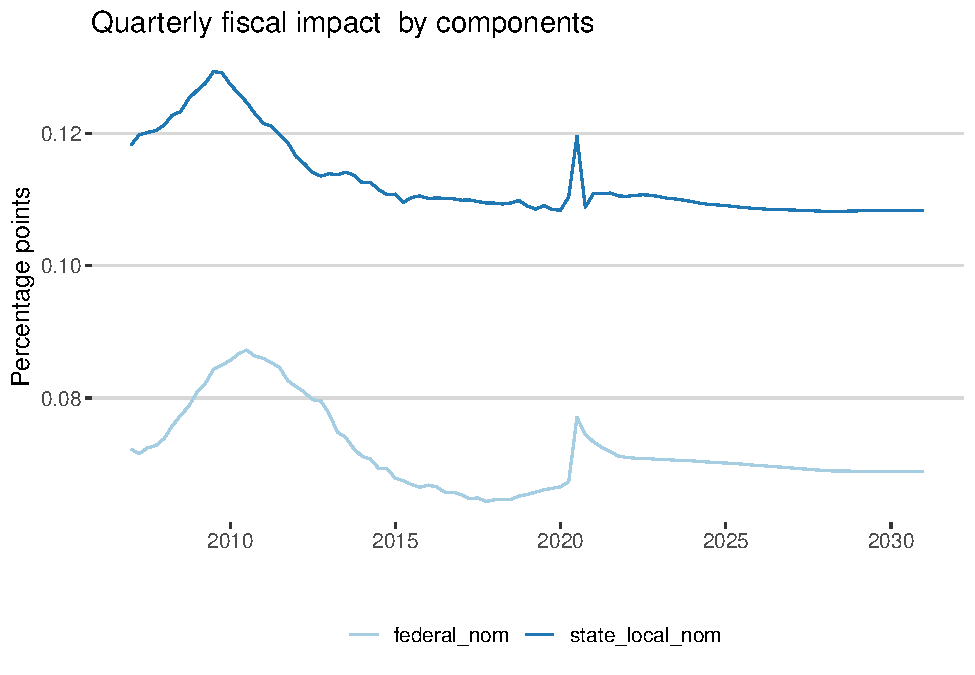
\includegraphics{projections_files/figure-latex/consumption and investment-1} \end{center}

\begin{verbatim}
## Warning: Removed 2 row(s) containing missing values (geom_path).
\end{verbatim}

\begin{center}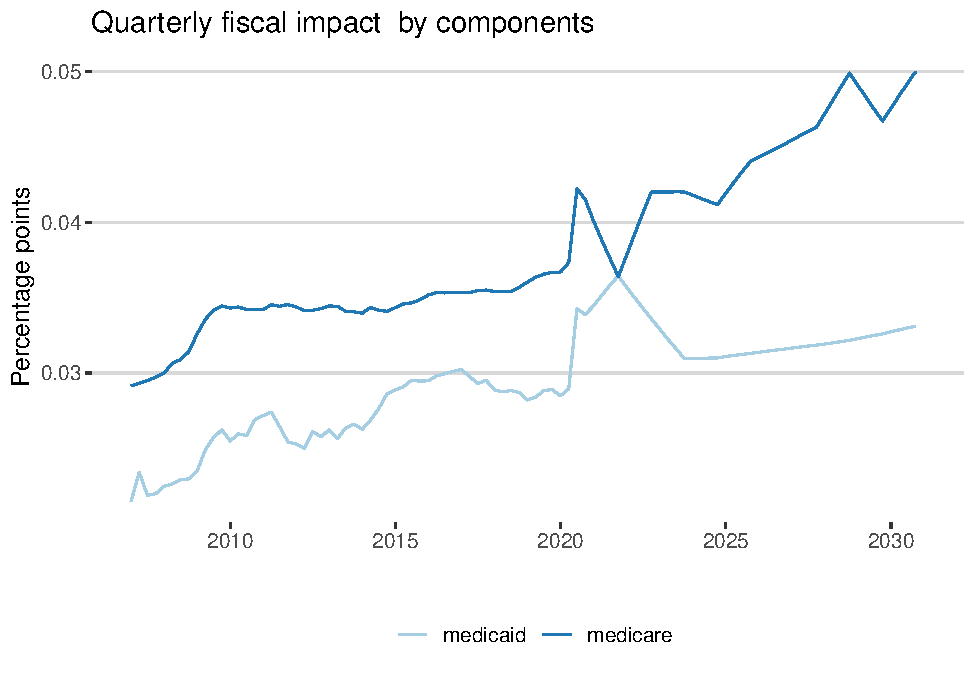
\includegraphics{projections_files/figure-latex/health-1} \end{center}

\begin{verbatim}
## Warning: Removed 1 row(s) containing missing values (geom_path).
\end{verbatim}

\begin{center}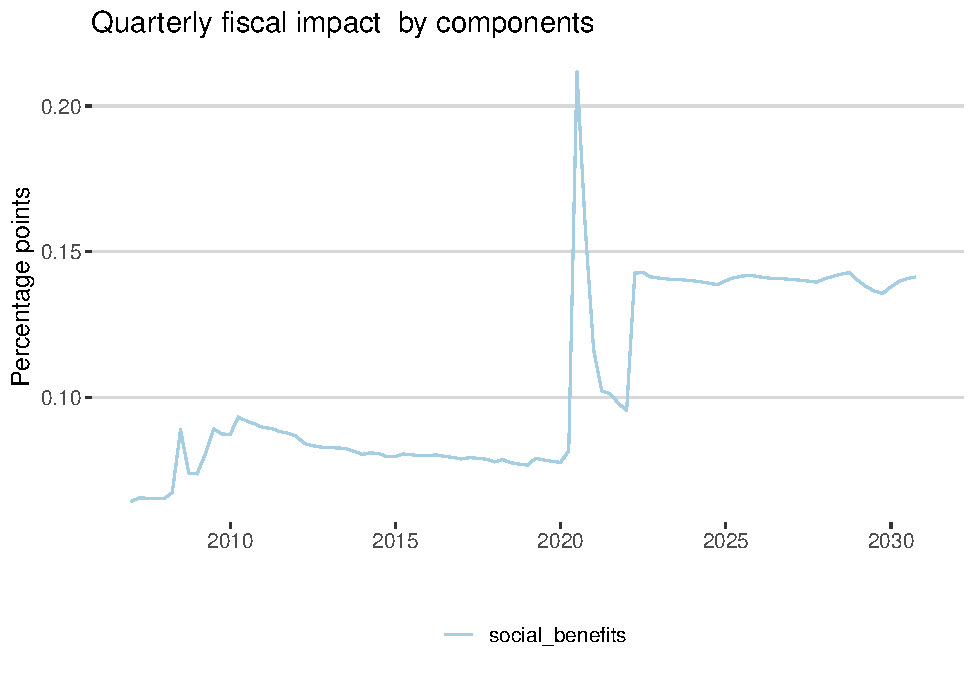
\includegraphics{projections_files/figure-latex/social benefits-1} \end{center}

\begin{verbatim}
## Warning: Removed 4 row(s) containing missing values (geom_path).
\end{verbatim}

\begin{center}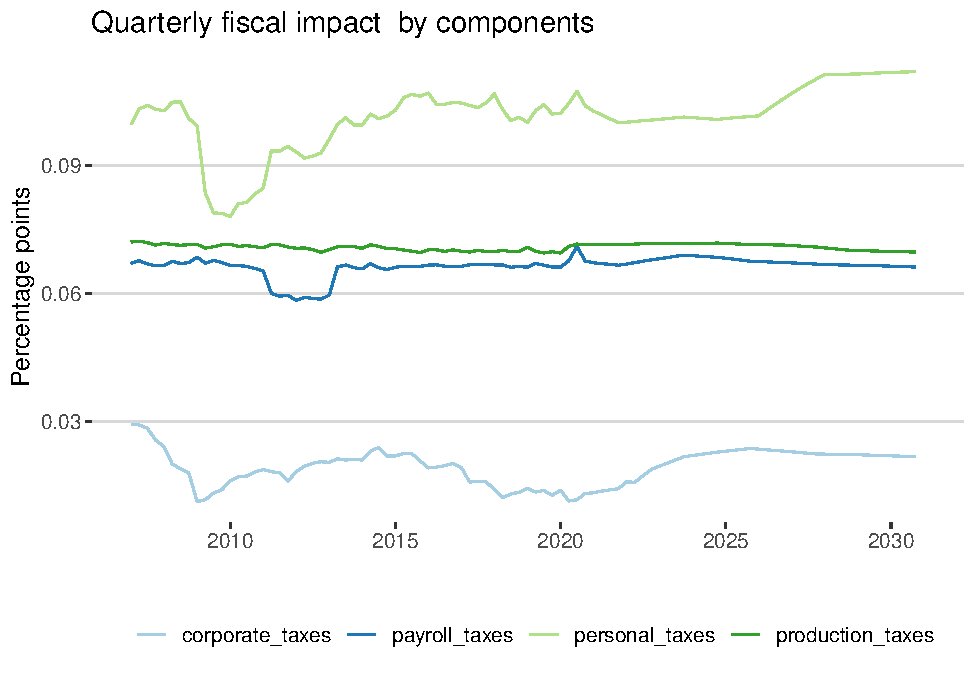
\includegraphics{projections_files/figure-latex/tax-1} \end{center}

\begin{verbatim}
## Warning: Removed 12 row(s) containing missing values (geom_path).
\end{verbatim}

\begin{center}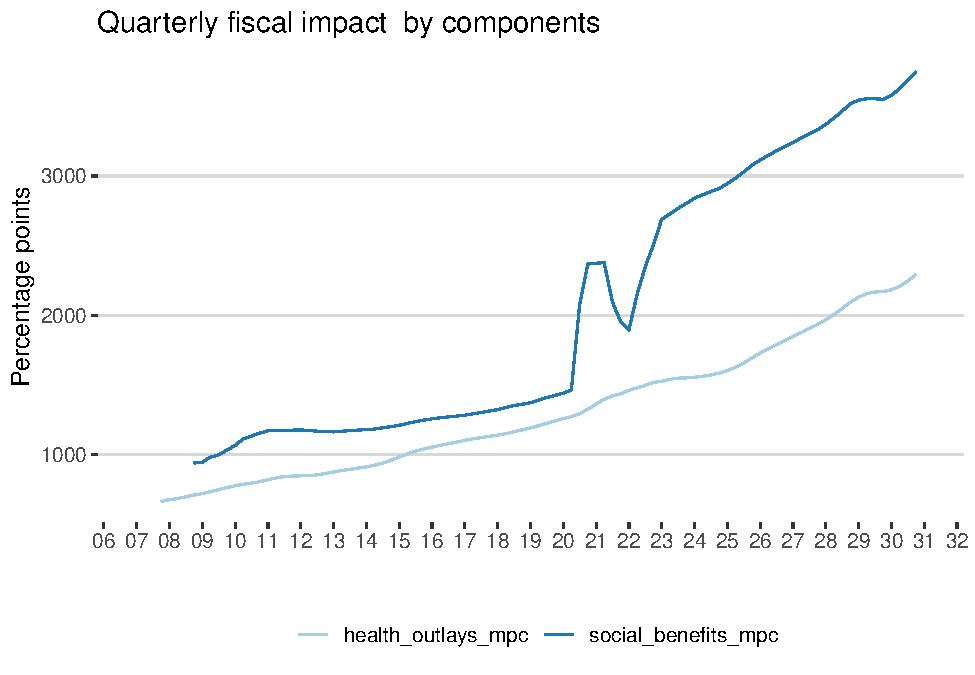
\includegraphics{projections_files/figure-latex/health consumption-1} \end{center}

\begin{verbatim}
## Warning: Removed 20 row(s) containing missing values (geom_path).
\end{verbatim}

\begin{center}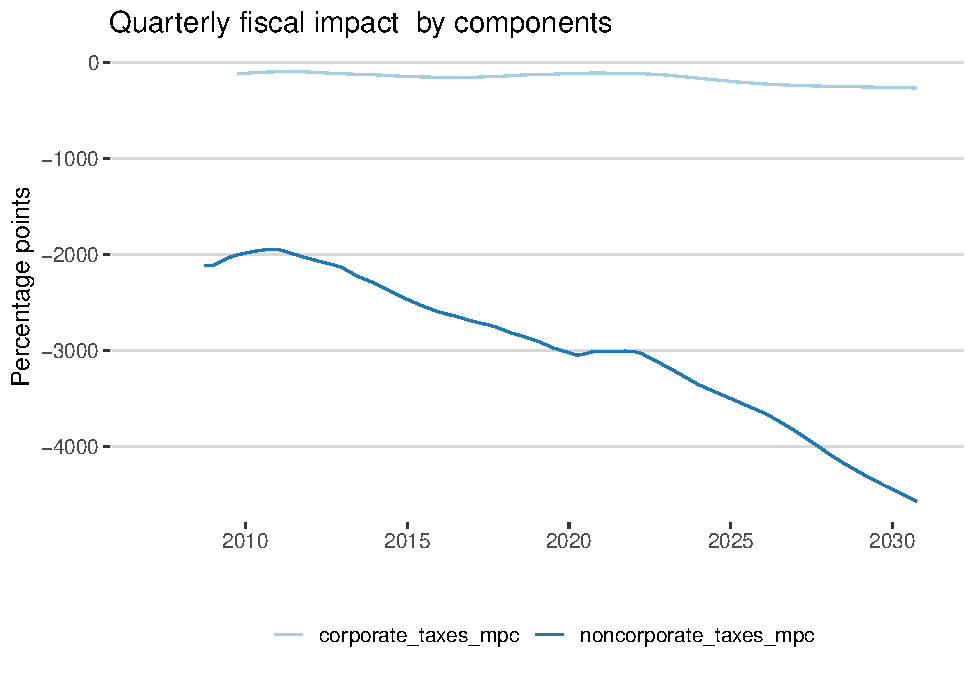
\includegraphics{projections_files/figure-latex/taxes consumption-1} \end{center}

\hypertarget{levels}{%
\subsection{Levels}\label{levels}}

\begin{center}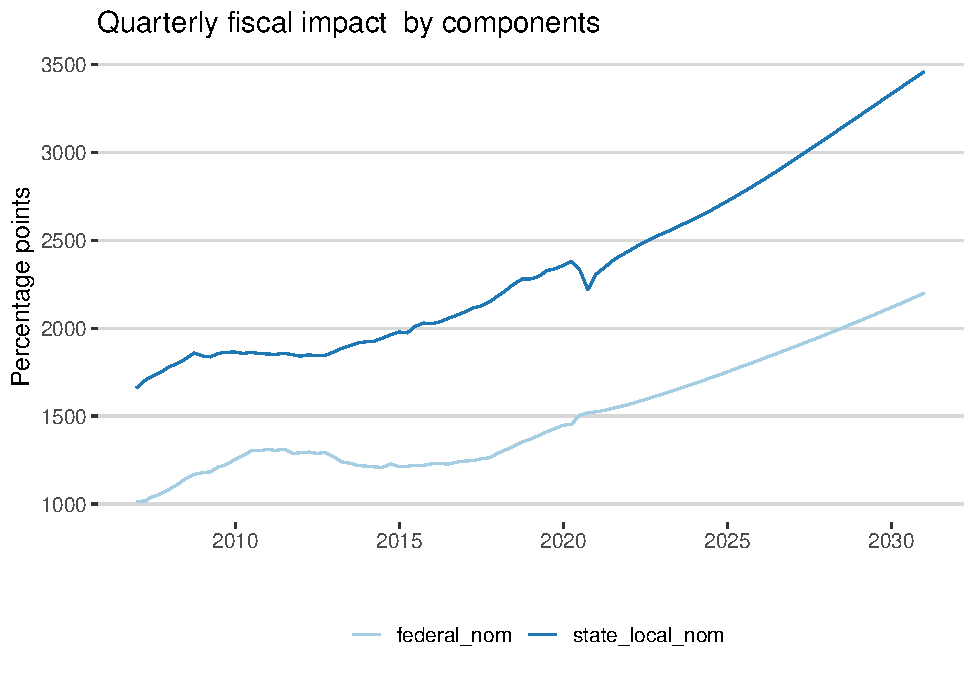
\includegraphics{projections_files/figure-latex/consumption and investment  levels-1} \end{center}

\begin{verbatim}
## Warning: Removed 2 row(s) containing missing values (geom_path).
\end{verbatim}

\begin{center}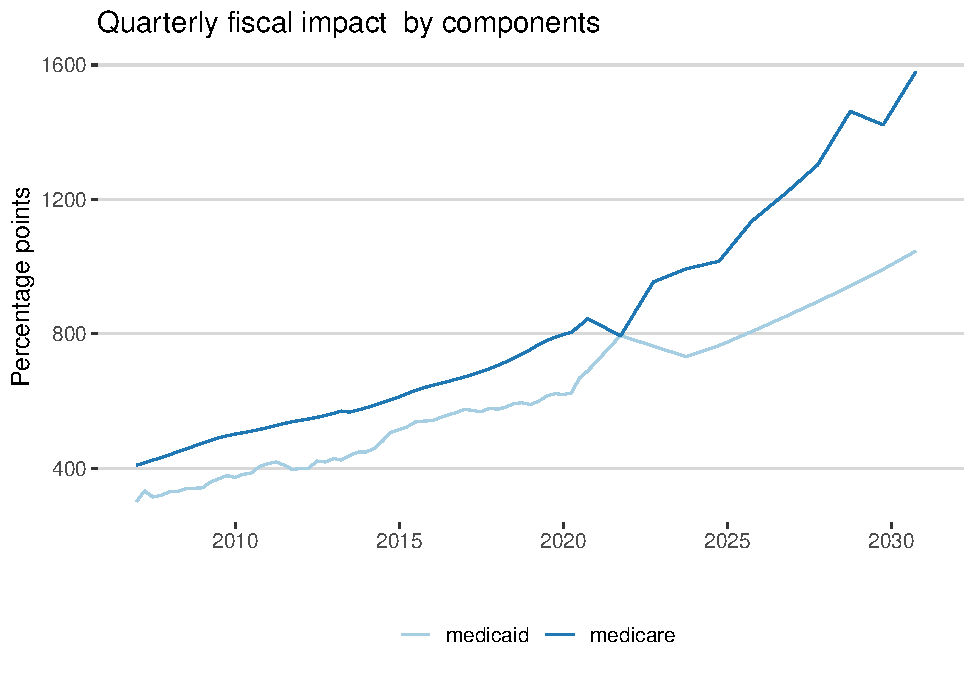
\includegraphics{projections_files/figure-latex/health levels-1} \end{center}

\begin{verbatim}
## Warning: Removed 1 row(s) containing missing values (geom_path).
\end{verbatim}

\begin{center}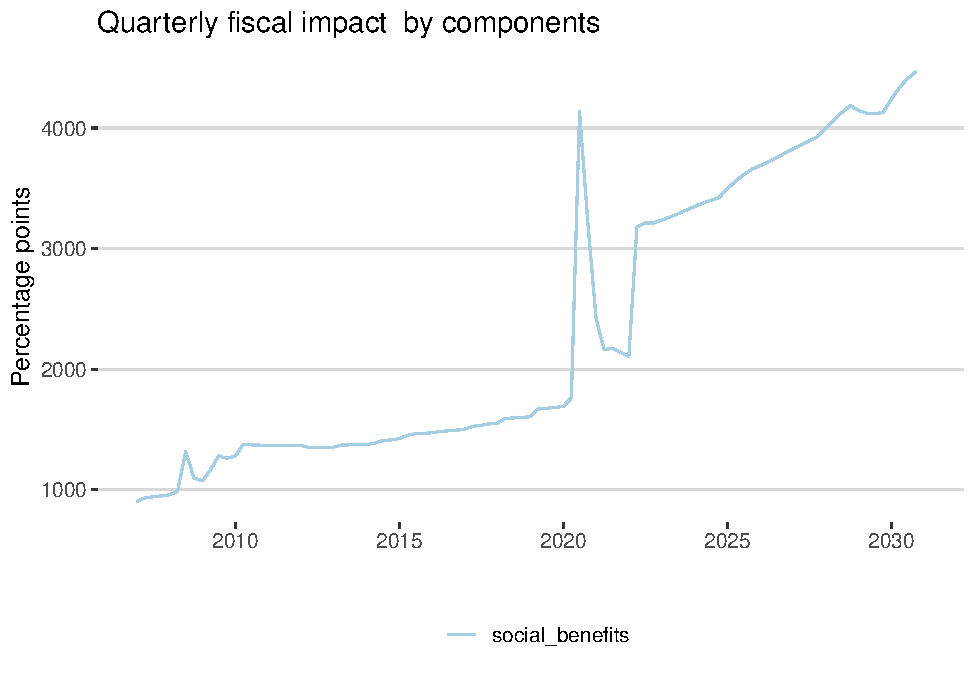
\includegraphics{projections_files/figure-latex/social benefits levels-1} \end{center}

\begin{verbatim}
## Warning: Removed 4 row(s) containing missing values (geom_path).
\end{verbatim}

\begin{center}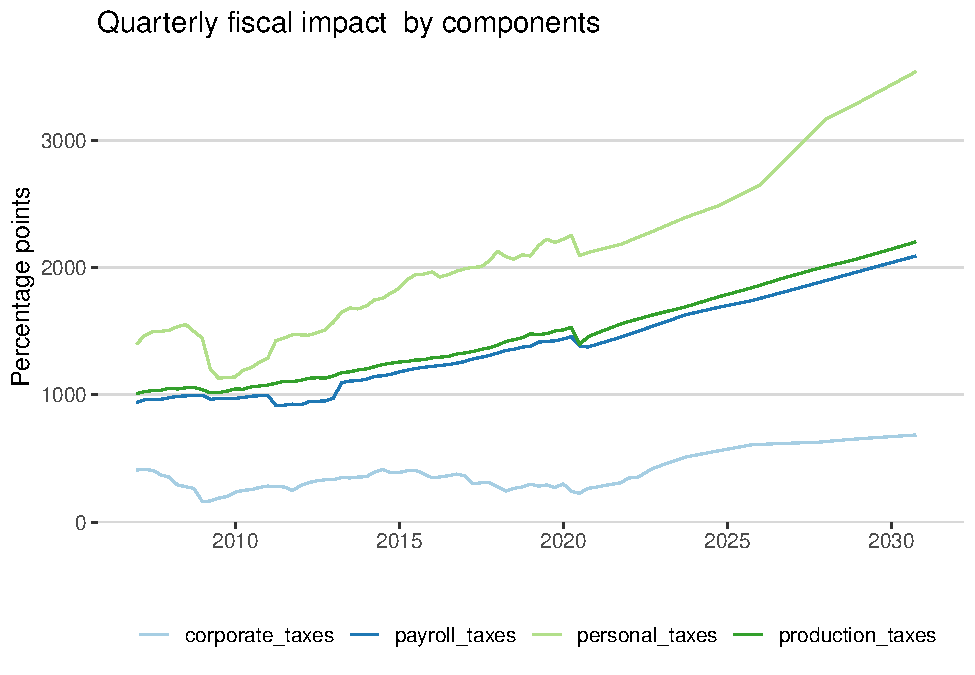
\includegraphics{projections_files/figure-latex/tax levels-1} \end{center}

\end{document}
